
\documentclass[11pt,a4paper,oneside]{report}
\usepackage{mathpazo} 
\linespread{1.05}        
\usepackage[scaled]{helvet} 
\usepackage{courier} 

\normalfont
\usepackage[T1]{fontenc}
\usepackage[footnotesize]{caption}
\usepackage{subfig}

\linespread{1.05}         

\parskip 7.2pt

\usepackage{setspace}
\onehalfspacing

\usepackage{framed}

\usepackage{pdfsync}
\sloppy

\setlength{\parindent}{0in} 


\usepackage[pdftex]{graphicx}

\usepackage{color}
\definecolor{gray09}{rgb}{0.9,0.9,0.9}  
\definecolor{red}{rgb}{1,0,0}
\definecolor{blue}{rgb}{0,0,1}
\definecolor{lightblue}{rgb}{0,0.8,1}
\definecolor{Dark}{gray}{.2}
\definecolor{Medium}{gray}{.6}
\definecolor{Light}{gray}{.8}
\definecolor{shadecolor}{rgb}{0.9, 0.9, 1}


\usepackage{epstopdf}

\usepackage{natbib}
\bibpunct{(}{)}{;}{a}{,}{,}

\usepackage{hyperref}
\hypersetup{colorlinks=true, 
	citecolor=blue, 
	linkcolor=blue, 
	urlcolor=blue}


\usepackage{fancyhdr}
\setlength{\headheight}{15.2pt}
\pagestyle{fancyplain}
\renewcommand{\chaptermark}[1]{\markboth{#1}{}}
\renewcommand{\sectionmark}[1]{\markright{\thesection\ #1}{}}
 
\lhead{\fancyplain{}{\textit{BIAS2015}}}
\chead{}
\rhead{\fancyplain{}{\textit{\rightmark}}}
\lfoot{}
\cfoot{\fancyplain{}{\thepage}}
\rfoot{}



\newenvironment{indentexercise}[1]
{{\setlength{\leftmargin}{2em}}
\textbf{Exercise \thesubsection-#1}
\begin{list}{}
	\item
}
{\end{list}}

\newenvironment{indentFiji}
{\begin{list}{}
         {\setlength{\leftmargin}{1em}}
         \item[]
}
{\end{list}}

\newenvironment{indentCom}
{\begin{list}{}
         {\setlength{\leftmargin}{1em}}
         \item[]
}
{\end{list}}

\newcommand{\ijmenu}[1]{\texttt{\small#1}}

\newcommand{\ilcom}[1]{\texttt{\small#1}}

 \newcommand{\tab}{\hspace*{3em}}

\newcommand{\HRule}{\rule{\linewidth}{0.5mm}}

\usepackage{textcomp}
\newcommand*{\micro}{\textmu}



\usepackage{listings}
\lstset{ 
basicstyle=\small\ttfamily, 
numbers=left,                   
numberstyle=\footnotesize,      
stepnumber=1,                   
numbersep=5pt,                  
backgroundcolor=\color{gray09},  
keywordstyle=\color{blue}, 	
showspaces=false,               
showstringspaces=false,         
showtabs=false,                 
tabsize=2,                      
captionpos=b,                   
breaklines=true,                
title=\lstname,                 
escapeinside={\%*}{*)},         
morekeywords={*,...},            
morecomment=[l]{//},
morecomment=[s]{/*}{*/},
morestring=[b]",
}



\newcommand*{\titleTH}{\begingroup
\raggedleft

\textsc{\textbf{\Large{Bias2015 \hfill Module 3}}} 
\HRule\\
\vspace*{\baselineskip}


\hfill \textsc{{\large Authors:}}\\
[0.3\baselineskip]
\hfill {\Large Ulrike Schulze}\\
{\small EMBL Heidelberg}\\
[0.3\baselineskip]
\hfill {\Large S\'{e}bastien Tosi}\\
{\small IRB Barcelona}\\
\vfill


{\textcolor{Medium}{\Huge FISH Spot Detection  in \\ Human Spermatozoids }}\\
[2\baselineskip]

{\bfseries BIAS2015 BioImage Data Analysis Course}\\
\textbf{EMBL Heidelberg}\\
\textbf{7-13 June 2015}

\vfill

\hfill\textsc{Reviewers/Teachers:}\\
[0.3\baselineskip]
{\large Perrine Paul-Gilloteaux}\\
{\small \hfill Institut Curie, Paris}\\
[0.3\baselineskip]
{\large \hfill Simon F. N\o rrelykke}\\
{\small \hfill ETH Z\"urich}\\
\HRule\\

{\small \hfill\textcolor{Medium}{ Compiled on: \today }}
\endgroup}



\begin{document}

\date{\today}
\pagestyle{empty}
\titleTH
\clearpage
\pagestyle{fancyplain}

\begingroup
\hypersetup{linkcolor=black}
\tableofcontents
\endgroup

\clearpage

\setcounter{chapter}{3}

\clearpage{}\setcounter{section}{-1} 
\newcounter{exerciseCounter} 
\setcounter{exerciseCounter}{1}

\section{Overview}

This module is divided into four separate steps. Each step has an enumerated workflow followed by an exercise. The result of each exercise is a macro. To ensure a smooth progress, the solution-macro for each exercise is provided and should be used as the starting point for consecutive exercises.

\subsection{Aim}

FISH (Fluorescent In-Situ Hybridization) is a complex gene staining technique with numerous variants \cite{volpi2008fish} where the quality of the staining depends on several physical parameters (e.g. level of DNA de-condensation). FISH aims at labeling DNA sequences specific to a certain gene (or chromosome) so that they appear as a "bright fluorescent spots" in fluorescent channels. We will write an ImageJ macro to process images from such a FISH assay: First to segment the spermatozoid nuclei from a DAPI staining, and then to classify the nuclei based on their chromosomal content (multiplicity of FISH spots in 3 different fluorescent channels).

\subsection{Introduction}

The automatic spermatozoids classification as proposed in \cite{molina2009fish} is a powerful mean to extract statistics of chromosomal anomalies (see Fig.~\ref{fig:intro}) on large sample datasets (typically >10'000 cells). It can also be used to drive a motorized microscope to perform an "intelligent" scan (\cite{tosi2012}): the classification is performed from a low resolution scan and a secondary scan (high resolution) is automatically triggered to only acquire the cells showing some specific anomalies.

\subsection{datasets}
The nuclei of the spermatozoids were DAPI stained and the chromosomes of interest (here X, Y and 18) were  stained by FISH. The fixed sample was scanned by a motorized stage microscope to tile the whole area of the sample. Several $z$ slices were recorded for each fluorescent channel (DAPI, aqua, orange, and green). The analysis will be performed on the z maximum intensity projection of the images (in each channel).

\begin{figure}[htbp]
\begin{center}
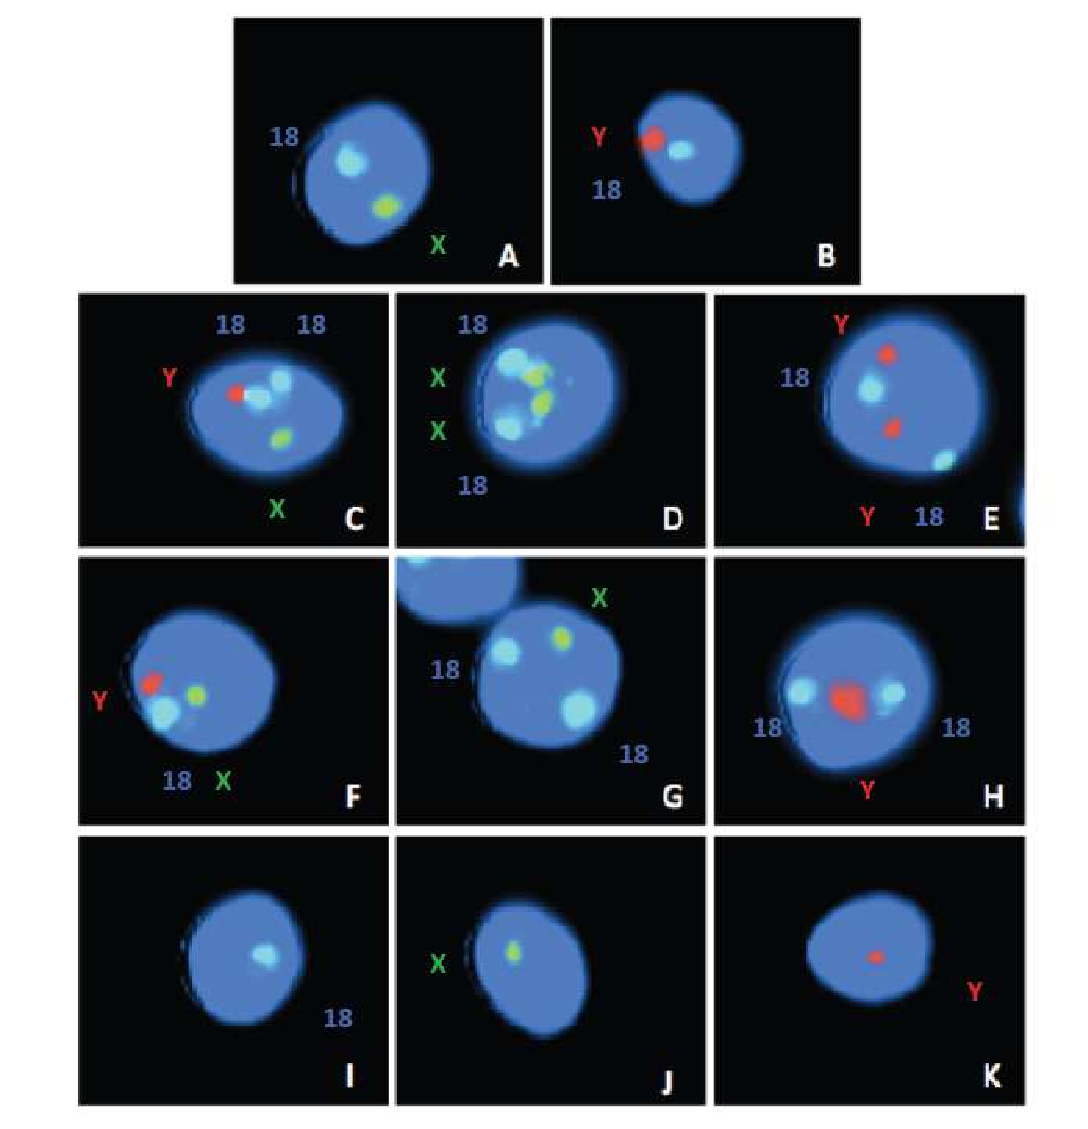
\includegraphics[width=3in]{fig/intro-eps-converted-to.pdf}
\caption{The upper cells are normal male and female spermatozoids, all the other cells are abnormal (Courtesy of Anna Godo, University of Barcelona).}
\label{fig:intro}
\end{center}
\end{figure}


\newpage
\section{Step 1: Initialization---a short warm-up}

\subsection{Workflow}

In Fiji, perform the steps described in this section with the command recorder open and create a macro from the recorder.
We will use the image \textbf{Small.tif}.\\

This hyperstack (4 channels) is a crop view from of a single field of a confocal dataset.
Each image is a maximum intensity projection, per channel, of the original data. 
The first image is a staining for the nuclei, all subsequent images are acquired in the fluorescence channels of the FISH stainings.

\begin{enumerate}
    \item Open the image file in Fiji by
    \ijmenu{[File > Open...]} or by drag and drop of the file on the Fiji bar.
    
    \item Examine the hyperstack using the stack browser (slider).
    
    \item Split Channels to get independent images for each fluorescence channel.
    \ijmenu{[Images > Color > Split Channels]}
    
    \begin{figure}[htbp]
        \centering
         \subfloat[]{\label{fig:SetScale}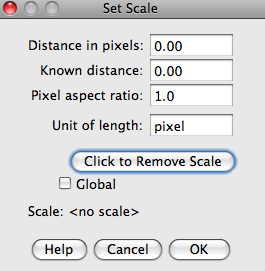
\includegraphics[width = 0.4\textwidth]{fig/SetScale.png}}
         \caption{Initialization}
         \label{fig:init}
    \end{figure}
    
    \item Remove the scale of the opened images by 
    \ijmenu{[Analyze > Set Scale\ldots]}. 
    Use the same settings as in Fig.~\ref{fig:init}:
    \begin{itemize}  
        \item\textbf{distance} and \textbf{known distance} to "0" and  
        \item\textbf{Pixel aspect ratio} to "1".  
        \item The \textbf{Unit length} should be "pixel". 
        \item  \textbf{Global} should be ticked so that the settings apply to all images (and subsequently opened images). 

    \end{itemize}

    Alternatively, press the "click to remove scale" button. 
    
    \item Set Binary Options 
    \ijmenu{[Process > Binary > Options...]}.
    Make sure "Iterations" and "Count" are both set to 1 and that "Black background" and "Pad edges when eroding" are NOT ticked. EDM output should be set to overwrite. These settings correspond to ImageJ default settings and it is a good habit to always set them to predictable values at the beginning of a macro since they control the behavior of many commands that are commonly used. 
    
    \item Set Measurements 
    \ijmenu{[Analyze > Set Measurements...]}.
    \begin{itemize}  
        \item\textbf{Area,} 
        \item\textbf{Mean gray value,}
        \item and \textbf{Shape Descriptors} 
        
        \item\textbf{Redirect} should be set to "None" 
        \item\textbf{Decimal places} should be 2 or greater.  
    \end{itemize} 

\end{enumerate}
\subsection{Exercise \arabic{exerciseCounter}}
\stepcounter{exerciseCounter}
Create a macro (from the recorder) that performs the steps 3 to 6 of the previous workflow.\footnote{If you are using OSX, it sometimes happens that copying from the command recorder and pasting it to the script editor does not work. In that case, try using right mouse click (or control-click) to copy recorded commands. If this still does not work, then click the ``Create'' button at the top-right corner.}. You can find the solution to the exercises as a complete macro in \textbf{code/solutions/module3\_01.ijm}.

\underline{\textbf{Note}}: We assume that the original hyperstack is already open when the macro is run.


\begin{lstlisting}[linerange={1-4}]
// Input: 
// - Hyperstack holding the 4 channels of the FISH assay (DAPI channel first)
// Output: 
// - Split channels, no scale

// Split channels
run("Split Channels");

// Initialization
run("Set Scale...", "distance=0 known=0 pixel=1 unit=pixel global");
run("Options...", "iterations=1 count=1 edm=Overwrite");
run("Set Measurements...", "area mean centroid shape redirect=None decimal=2");
\end{lstlisting}
\textbf{sourcecode}: \href{http://www.example.com/contents}{code/solutions/module3\_01.ijm}

It is a good habit to add a preamble to a macro holding author, purpose, version, date and any helpful additional notes. Comments should also be added throughout the macro to summarize the aim of specific sub-sections (e.g. ``Initialization'', ``Erase the small particles''), especially if the sequence of commands is not straightforward to understand. These comments will often prove useful to people reading your code and to yourself when reading the code to modify it years after.

\subsection{Summary of tools used in Step 1}

Here is a summary of the main ImageJ tools used in this step:

\begin{itemize}
\item \textbf{Split Channels} \ijmenu{[Images > Color > Split Channels]}.\\
Split channels to get independent images for each fluorescence channel.

\item \textbf{Set Scale} \ijmenu{[Analyze > Set Scale...]}.\\
Allow to calibrate the pixel size

\item \textbf{Binary Options} \ijmenu{[Process>Binary> Options...]}.\\ 
Set the behavior of binary image related commands.

\item \textbf{Set Measurements} \ijmenu{[Analyze > Set Measurements...]}.\\ 
Set which features should be measured when calling \ijmenu{[Analyze > Measure]}.
\end{itemize} 



\newpage
\section{Step 2: Segment Nuclei}

Here, we will segment the nuclei in the image of the first channel \textbf{"C1-Small.tif"}. We would like to ignore deformed (Fig.~\ref{fig:NucDeformed}) and unusually small (Fig.~\ref{fig:NucSmall}) or large nuclei. In addition, the algorithm should identify touching nuclei (Fig.~\ref{fig:NucTwo}) so that these clusters are either ignored or properly split.

\subsection{Workflow}

We will first perform some manual processing on the image of the first channel to understand each step. After this we write a macro to perform these operations automatically (see Module 2 for an introduction of the macro programming language). Leave the command recorder open to record operations as you manually perform them.

\begin{enumerate}
    \item Select Image (make window active). 
    In Step 1 we split the channels of the original hyperstack. Now we have four independent images. To process the nuclei channel image we need to make it "active" by clicking on its window: make \textbf{"C1-Small.tif"} active.
    
    \underline{\textbf{Note}}: To select an image from a macro, we use the function \textbf{selectImage("name")} where "name" is the name of the image window. 
    Alternatively the identifier (ID) of an image can be passed to \textbf{selectImage()}. 
    This ID must first be retrieved by calling \textbf{getImageID()} at a step where the image is known to be "active".
    
    \begin{figure}[htbp]
        \centering
         \subfloat[nicely shaped]{\label{fig:NucGood}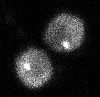
\includegraphics[height = 0.12\textheight]{fig/NucGood.png}} 
        \quad
         \subfloat[small ]{\label{fig:NucSmall}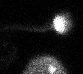
\includegraphics[height = 0.12\textheight]{fig/NucSmall.png}} 
         \quad
         \subfloat[some merged nuclei]{\label{fig:NucTwo}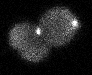
\includegraphics[height = 0.12\textheight]{fig/NucTwo.png}} 
         \quad
          \subfloat[deformed ]{\label{fig:NucDeformed}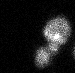
\includegraphics[height = 0.12\textheight]{fig/NucDeformed.png}} 
         \caption{Typical images of nuclei in the DAPI channel}
         \label{fig:nucleiShapes}
    \end{figure}
    
    \item Apply ``Laplacian of Gaussian'' (see Sec.~\textbf{Convolution} of Module~1 for an introduction to convolution filters ). We use a Laplacian of Gaussian (Log) filter as a preprocessing step to facilitate the segmentation (see section \ref{summary_of_tools_mod_3_step_2} for more information about the Log filter). In ImageJ this filter can be found in \ijmenu{[Plugins > Feature Extraction> FeatureJ > FeatureJ Laplacian]}.
    
    The first step of the filter is a Gaussian filter whose radius (smoothing scale) must be adjusted to the typical size of the nuclei. The next step is a Laplacian filter. When the smoothing scale is properly adjusted the nuclei appear as homogeneously dark and surrounded by a bright halo in the filtered image (see Fig.~\ref{fig:nucleiLaplacian}(b)). A rule of thumb is to set the smoothing scale to about half the expected radius of the objects. 
    
    Note, that the output of the filter is a 32 bit image since the intensity values can be negative or positive. FeatureJ Laplacian can also detect zero-crossings, where the intensity changes sign (close to a sharp intensity transition), but we will not use this feature here (leave unticked). Make sure that "Compute Laplacian image" is ticked.
    
    To better understand the advantage of using a Laplacian prefiltering, you can try to directly apply a threshold on the original nuclei image.

    \begin{figure}[h!tbp]
        \centering
         \subfloat[before]{\label{fig:NucBeforeLaplacian}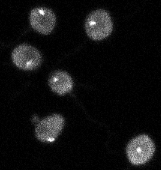
\includegraphics[height = 0.18\textheight]{fig/NucBeforeLaplacian.png}} 
        \quad
         \subfloat[after ]{\label{fig:NucAfterLaplacian}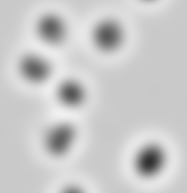
\includegraphics[height = 0.18\textheight]{fig/NucAfterLaplacian.png}} 
         \quad
          \subfloat[after applying a special LUT ("6\_shades") to show the iso-intensity levels]{\label{fig:NucAfterLaplacianLUT}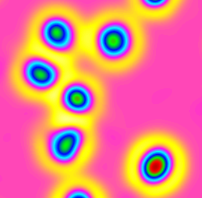
\includegraphics[height = 0.18\textheight]{fig/NucAfterLaplacianLUT.png}} 
         \caption{Image before and after application of FeatureJ Laplacian}
         \label{fig:nucleiLaplacian}
    \end{figure}

In Fig.~\ref{fig:nucleiLaplacian} we can observe the result of the LoG filter performed on the nuclei image. The shapes of the nuclei are nicely mimicked in rings of different intensities (Fig.~\ref{fig:NucAfterLaplacianLUT}), as it can be visualized by changing the LUT to a colored LUT (\ijmenu{[Image> LookUp Tables]} to get the list of available LUTs). Try to optimize the smoothing scale of FeatureJ Laplacian to obtain a result similar to \ref{fig:nucleiLaplacian}.

    \item Set threshold and convert to mask. 
    Here, we will convert this image into a binary image by thresholding (see section on \textbf{thresholding} in Module 1). We need to set the bounds of the threshold to separate the nuclei from the background. To achieve this, we use the command:
   
    \ijmenu{[Image >  Adjust > Threshold...]}
    
    Make sure to un-tick "Dark Bakground" and "set background pixels to NaN" (appears as pop-up window when clicking "Apply"), to obtain a regular 8-bit binary image (mask). Thanks to the preprocessing the nuclei can now readily be segmented by thresholding the pixels with negative values (up to a small negative value) in the filtered image. 
    The results is a black and white image, in which all pixels that belong to an object have an intensity value of 255, while all pixels that belong to the background have an intensity value of 0. 
    
    \textbf{\underline{Note}}: After converting the image to binary ImageJ automatically applies (by default) a LUT inversion: The objects now appear black on a white background. See also  \url{http://imagej.nih.gov/ij/docs/guide/146-29.html#infobox:InvertedLutMask}
    

    \item Fill holes
    \ijmenu{[Process >  Binary > Fill Holes]}.
    Some objects of the binary image might have holes (see Fig.~\ref{fig:NucFillHoles}). A hole is defined as a group of pixels belonging to the background (white pixels) surrounded by pixels belonging to the foreground (black pixels). Since we do not expect the nuclei to exhibit any hole, we use \ijmenu{[Process > Binary > Fill Holes]} to fill them in (see section \textbf{Morphology} in Module 1).
    
    \begin{figure}[h!tbp]
        \centering
         \subfloat[before]{\label{fig:NucBeforeFillHoles}
\includegraphics[height = 0.18\textheight]{fig/NucBeforeFillHoles.png}} 
        \quad
         \subfloat[after ]{\label{fig:NucAfterFillHoles}
\includegraphics[height = 0.18\textheight]{fig/NucAfterFillHoles.png}} 
         \quad
         \caption{Image before and after application of Fill Holes (image video inverted)}
         \label{fig:NucFillHoles}
    \end{figure}
    
    \item Dilate
    \ijmenu{[Process >  Binary > Dilate]}.
    From Fig.~\ref{fig:NucOverlayBeforeDilate} we can see that the detected boundaries mostly follow the contours of the nuclei but that they sometimes overlap with them. This may become a problem later on when intending to detect a FISH spot close to the boundary of a nucleus. This problem can be mitigated by enlarging the segmented nuclei by morphological dilation (see section \textbf{Morphology} in Module 1). Each round of dilation enlarges the objects by one pixel, several dilations can be performed sequentially. 
    
\begin{figure}[htbp]
\centering
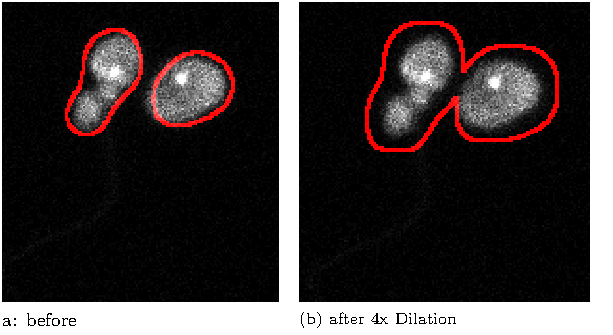
\includegraphics[width=3in]{mod3mergedfig-NucOverlayDilate.pdf}

         \caption{Overlay of original image and segmented binary image before and after several dilations (for better visibility only the boundaries of the segmented images are represented)}

         \label{fig:NucOverlayDilate}
    \end{figure}


    \item Watershed
    \ijmenu{[Process >  Binary > Watershed]}.
    Try the binary watershed command to separate touching nuclei.
    
    \begin{figure}[htbp]
        \centering
         \subfloat[before]{\label{fig:NucBeforeWatershed}
\includegraphics[height = 0.18\textheight]{fig/NucBeforeWatershed.png}} 
        \quad
         \subfloat[after]{\label{fig:NucAfterWatershed}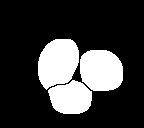
\includegraphics[height = 0.18\textheight]{fig/NucAfterWatershed.png}} 
         \quad
         \caption{Separating nuclei with watershed (image video inverted)}
         \label{fig:NucWatershed}
    \end{figure}

    \item Analyze Particles.
    At this point we obtained a binary image holding the segmented nuclei.
    Using \ijmenu{[Analyze > Analyze Particle]} we can identify and measure several properties of these connected particles. This command also allows us to exclude an object based on its geometry. For our purpose,  we want to exclude deformed particles and particles that are too small or too big.
    
    To exclude deformed particles, we can measure their circularity. The circularity describes how closely an object resembles a circle by computing the ratio between its area and its square perimeter. A perfect circle has a circularity parameter = 1. Any other object will have a circularity parameter smaller than 1, but greater than 0 (an infinite line). 
    
    Particles that are smaller or larger than given critical areas can also be excluded. The area bounds should be first determined empirically: you can do so by measuring the area of a typical nucleus and setting the lower and upper bounds to, for instance 0.66x and 1.5x this value. 
    
    Finally, particles touching a border can be easily discarded by ticking "Exclude on edges" in \ijmenu{[Analyze > Analyze Particles...]}. The purpose is to analyse FISH spots by nucleus, do not forget to also tick 'Add to Manager' to add the nuclei analyzed to the ROI Manager so that they can easily be accessed further on.
    

\end{enumerate}
\subsection{Exercise \arabic{exerciseCounter}}
\stepcounter{exerciseCounter}
Following the workflow described above write a macro to segment the nuclei in the image \textbf{"C1-Small.tif"}. The solution to this exercise is provided in: \textbf{code/solutions/module3\_02simple.ijm}.

\textbf{\underline{Note}}: The lower bound of the threshold should be set to the minimum intensity of the image, search for a macro function allowing to retrieve this value.
\subsection{Exercise \arabic{exerciseCounter}}
\stepcounter{exerciseCounter}

The lower and upper bounds of the nuclei area have been so far empirically set, we will now automate the estimation of these bounds. For this we will first analyze the particles after thresholding without setting any area bounds (do not add the particles to the ROI manager at this point). The areas of the analyzed particles will be measured to results table and copied to an array to be further processed (this can be done by writing a loop). Assuming that valid nuclei are in majority, try to figure out a way to estimate the lower and higher area bounds from the area measurements. Finally we will analyze the particles again but this time setting lower and upper area bounds (and adding them to the ROI manager).\\

\textbf{\underline{Hint}}: A useful function that we will make use of is \textbf{Array.sort(MyArray)}. The median can be computed by sorting the n areas and selecting the n/2$^{th}$ area.\\
 
Using this technique we can analyze images that have been taken with a wide variety of magnifications without having to manually adapt the "typical" area. You can find the solution to both exercises as a complete macro in \textbf{code/solutions/module3\_02.ijm}.



\begin{lstlisting}[linerange={1-4}]
// Input: 
// - 4 channels of the FISH experiment in 4 images: C1-Small.tif, C2-Small.tif, C3-Small.tif and C4-Small.tif
// Output: 
// - Detected nuclei in ROI manager

//Segment Nuclei
selectImage("C1-Small.tif");
run("FeatureJ Laplacian", "compute smoothing=12");
getMinAndMax(min,max);
setThreshold(min,-0.05);
run("Convert to Mask");
run("Fill Holes");
for(i=0;i<2;i++)run("Dilate");

//Split Particles
run("Watershed");
rename("Mask");

//Analyze particle to estimate median area
run("Analyze Particles...", "size=0-Infinity circularity=0.75-1.00 show=Nothing display exclude clear include"); 
Area = newArray(nResults);
for(i=0;i<nResults;i++)Area[i] = getResult("Area", i);
Area = Array.sort(Area);
MedianArea = Area[nResults/2];
print("Median area: "+d2s(MedianArea,0));

//Analyze Particles and store to ROI manager
run("Analyze Particles...", "size="+MedianArea*0.66+"-"+MedianArea*1.5+" circularity=0.75-1.00 show=Nothing display exclude clear include add");
NbNuclei = roiManager("count");

selectImage("Mask");
close();
selectImage("C1-Small.tif");
roiManager("Show All");
\end{lstlisting}
\textbf{sourcecode}: \href{http://www.example.com/contents}{code/solutions/module3\_02.ijm}

\subsection{Summary of tools used in Step 2}
\label{summary_of_tools_mod_3_step_2}
\begin{itemize}

\item \textbf{FeatureJ Laplacian}\\
\ijmenu{[Plugins > Feature Extraction > FeatureJ > FeatureJ Laplacian]}.\\
\url{http://imagescience.org/meijering/software/featurej/}\\
 After applying a Gaussian filter with radius defined by the smoothing scale this command computes the sum of the second order spacial derivatives of the intensity along the Cartesian directions at each pixel. \\
It is used to emphasize large isotropic intensity curvature (domes) in an image. This combination of filters (Gaussian followed by Laplacian) is called "LoG" for Laplacian of Gaussian and is commonly used for spot or blob enhancement. The optimal smoothing scale is directly related to the radius of the blob-like objects to be enhanced. The LoG is ubiquitous in image processing and was popularized by \cite{lindeberg1993scale} for feature detection in the framework of the scale-space theory.

\item \textbf{Convert to Mask} \ijmenu{[Image > Binary > Convert to Mask]}.\\
Convert a gray-scale image into a binary (black and white) image, the active threshold is used to define whether a pixel is part of the foreground or of the background. 

\item \textbf{setThreshold} \ijmenu{[Image > Adjust > Threshold ...]}.\\
Set the values of the threshold bounds.

\item \textbf{Fill Holes} \ijmenu{[Process > Binary > Fill Holes]}.\\
Fill holes in the connected particles (objects) of a binary image. 

\item \textbf{Analyze Particles}  \ijmenu{[Analyze > Analyze Particles...]}.\\
Find the connected particles in a binary image and optionally filter them (keep/discard) based on their area, geometric properties or location (touching an edge of the image).

\item \textbf{Dilate} \ijmenu{[Process > Binary > Dilate]}.\\
Enlarge the objects in a binary image. This command enlarges the boundaries of the objects by one pixel. 

\item \textbf{Watershed} \ijmenu{[Process > Binary > Watershed]}.\\
Intent to split touching/overlapping particles to individual particles in a binary image.
\end{itemize}
 
 
\newpage
\section{Step 3: FISH spots detection} 

Again we will perform a sequence of image processing steps manually and then include them in a macro. The starting point is to have the channels split and the nuclei stored in the ROI manager (if you lose the information at any time you can sequentially launch the macros from Steps 1 and 2 on the original hyperstack to get to this point).

\subsection{Workflow}
In this section we will segment all the spots in the three FISH channels. To detect the spots we use a similar prefiltering as for the segmentation of the nuclei (with a different smoothing scale).

\begin{enumerate}
    \item Apply Laplacian of Gaussian. We pre-filter the image of the first FISH channel with \ijmenu{[Plugins > Feature Extraction > FeatureJ >  FeatureJ Laplacian]}. The smoothing scale should be adjusted to the size of the spots! 
    \begin{figure}[htbp]
        \centering
        \subfloat[before]{\label{fig:Ch3BeforeLaplacian}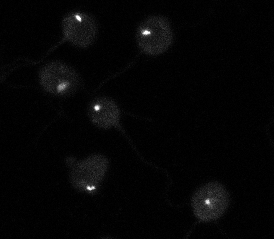
\includegraphics[height = 0.18\textheight]{fig/Ch3BeforeLaplacian.png}} 
        \quad
        \subfloat[after]{\label{fig:Ch3AfterLaplacian}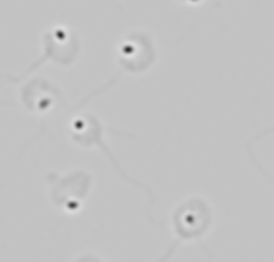
\includegraphics[height = 0.18\textheight]{fig/Ch3AfterLaplacian.png}} 
        \quad
        \caption{A FISH channel before and after applying the LoG filter}
\end{figure}
    
    \item Detect intensity regional minima with \ijmenu{[Process > Find Maxima...]}. You should tick \textbf{"Light background"} to detect minima and adjust \textbf{"Noise tolerance"} to optimize detection. Select \textbf{"Single Points"} as \textbf{"Output Type"} to create a binary mask with detected minima.
    
    \item Counting spots inside nuclei.
    In Step 2 we have already segmented the nuclei and stored them to the ROI manager. Now, we simply need to select the binary mask holding the detect spots and loop through the nuclei ROIs. Next, we count the number of pixels with intensity equal to 255 to retrieve the number of spots per nucleus.
    
    For each nucleus we will measure the statistics of the intensity with the macro function \textbf{getRawStatistics(nPixels, mean, min, max, std, histogram)} which among other returns the histogram of the pixel intensity inside the active selection. 

\end{enumerate}

\subsection{Exercise \arabic{exerciseCounter}}
\stepcounter{exerciseCounter}
Complete the macro \textbf{code/module3\_03simple-incomplete.ijm} to perform the previous sequence on the three FISH channels. Before launching the macro you need to have \textbf{C2-Small.tif} opened and the detected nuclei stored in the ROI Manager.

Open, read, and test the macro. The macro automatically segments the FISH spots following the workflow we previously described but the part counting the spots in each nucleus is incomplete. Several tasks have to be performed:

\begin{enumerate}

\item Write the missing code to detect the intensity regional minima. If you perform it right you should see a list of values indicating the number of spots detected in each nucleus in the log window. Solution in \textbf{code/solutions/module3\_03simple.ijm}.

\item Modify the code to automatically repeat the same workflow on the other 2 channels. This time you need the 3 channels opened before running the code. Solution in \textbf{code/solutions/module3\_03.ijm}.
\end{enumerate}

\textbf{\underline{Hint}}: You will need a loop over the channels. To properly select the correct image at each iteration you can make use of string concatenation (the channel images are called \textbf{"C2-Small.tif"}, \textbf{"C3-Small.tif"} and \textbf{"C4-Small.tif"}).


\begin{lstlisting}[linerange={1-6}]
// Input: 
// - ROI Manager with nuclei selection
// - C1-Small.tif, C2-Small.tif, C3-Small.tif and C4-Small.tif opened
// Output: 
// - Spot segmentation masks of the 3 channels
// - 3 Arrays (on per channel) with spot counted in each nucleus

NbNuclei = roiManager("count");

// FISH spots detection
NbSpotsChan1 = newArray(NbNuclei);
NbSpotsChan2 = newArray(NbNuclei);
NbSpotsChan3 = newArray(NbNuclei);
for(i=1;i<4;i++)
{
	// Pre-filtering
	selectImage("C"+d2s(i+1,0)+"-Small.tif");
	run("FeatureJ Laplacian", "compute smoothing=3");
	SpotLapID = getImageID();
	
	// Spot segmentation
	run("Find Maxima...", "noise=4 output=[Single Points] light");
	SpotCandMaskID = getImageID();

	// Cleanup
	selectImage(SpotLapID);
	close();
	
	// Spot count in each nucleus
	selectImage(SpotCandMaskID);
	for(j=0;j<NbNuclei;j++)
	{ 	
		roiManager("select",j);
		getRawStatistics(nPixels, mean, min, max, std, histogram);
		NbSpots = histogram[255];
		if(i==1)NbSpotsChan1[j] = NbSpots;
		if(i==2)NbSpotsChan2[j] = NbSpots;
		if(i==3)NbSpotsChan3[j] = NbSpots;
	}
	
}
run("Select None");

// Display arrays with counted spots per nucleus
print("Array NbSpotsChan1:");
Array.print(NbSpotsChan1);
print("Array NbSpotsChan2:");
Array.print(NbSpotsChan2);
print("Array NbSpotsChan3:");
Array.print(NbSpotsChan3);
\end{lstlisting}
\textbf{sourcecode}: \href{http://www.example.com/contents}{code/solutions/module3\_03.ijm}

\subsection{Summary of tools used in Step 3}
\begin{itemize}
\item\textbf{FeatureJ Laplacian} See step 2

\item\textbf{Threshold} See ``ImageJ Basics''.
\item\textbf{Analyze Particles} See ``ImageJ Basics''.
\item\textbf{ROI Manager} See ``ImageJ Basics''.

\end{itemize}


\newpage
\section{Step 4: Visualization (making it look pretty)}
\subsection{Workflow}
In this section we will visualize the nuclei and spots previously detected by overlaying them to the original image. The spot markers should be color coded according to their channel and the nuclei boundaries should be color coded according to the number of FISH spots detected in each FISH channel.
\begin{figure}[htbp]
    \centering
     \subfloat[]{\label{}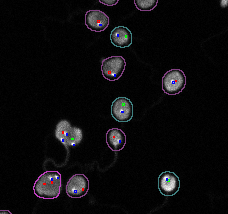
\includegraphics[height = 0.3\textheight]{fig/VisColorCode.png}} 
     \caption{All analyzed nuclei are marked with a color code depending on the number and type of FISH spot found inside them}
     \label{fig:VisGoal}
\end{figure}

\begin{enumerate}
    \item Overlaying the FISH spots on the original image.
    Select "SpotCandidates", the binary image holding the detected spots, threshold the image and then call \ijmenu{[Edit > Selection > Create Selection]}. The selection can then be transferred (restored) to another image using \ijmenu{[Edit > Selection > Restore Selection]} or saved to the ROI manager. To make the spots more visible, we increase their size in the selection with \ijmenu{[Edit > Selection > Enlarge... ]}. You can try to restore the selection on the original image to check the accuracy of the detection.

    \item Coloring the nuclei according to number and type of FISH spots.
    
    The color of the nuclei should be set according to their multiplicity of spots. For example, a nucleus with two red spots and two blue spots should have a different color than a nucleus with one red spot and one green spot.
    
    To achieve this, we take advantage from the fact that all colors are displayed as a combination of red, green and blue. How much of red, green and blue is used for a color is described by a number from 0 to 255. This number is written as a hexadecimal number (from 00 to FF). In this system white is coded as FFFFFF (red: intensity 255, green: intensity 255, blue: intensity: 255). Black is coded as 000000 (red:0, green:0, blue:0). Pure red would be coded as FF0000 (red: 255, blue:0, green:0) and purple would be coded as FF00FF (red: 255, green:0, blue: 255).
    
    To color the nuclei we will loop again through their selections in the ROI manager and assign them a specific stroke color depending on the spot counts. As we do not expect the number of spots to exceed 2 per nucleus the color will be simply defined as follow:
    
    red: 63+64*Number of spots in channel 1\\
    green: 63+64* Number of spots in channel 2\\
    blue: 63+64 * Number of spots in channel 3.
    
\end{enumerate}

\subsection{Exercise  \arabic{exerciseCounter}}
\stepcounter{exerciseCounter} 
Starting from the macro \textbf{code/module\_03.ijm} and following the steps described in the section "Marking the FISH spots" add the missing code to show an overlay of the detected spots (store the selection to the ROI manager with \ijmenu{[Edit > Selection > Add to Manager}]). The code should be added at the end of the loop over the FISH channel.

\underline{\textbf{Hint}}: You should start by reducing the upper limit of the loop so that only the first channel is processed. Then only try to make your macro run over the three channels (this is a typical debugging trick). 

Now try to implement the steps of the section "Marking the nuclei according to number and type of FISH spots".

\underline{\textbf{Hint}}: To change the color of a selection of the ROI Manager you will have to select it first with \textbf{roiManager("select", ...)} then call \ijmenu{Edit > Selection > Properties} and update the selection in the ROI Manager with \textbf{roiManager("update")}. To understand the parameters that should be passed to the command record it and input a stroke color of the type FFxxxxxx where the xx stands for each of the three hexadecimal values of the RGB color channels (the first field codes the transparency, we set it to FF which is equivalent to non transparent). 

\underline{\textbf{Note}}:The macro function \textbf{toHex} converts a decimal number to its hexadecimal representation.

Finally open the solution \textbf{code/solutions/module3\_03-04.ijm} to the previous exercise and test it. As you will notice the overlay of the spots is not associated to the slice (channel) in which they were detected but they all appear simultaneously. By un-commenting the last section of the code you can modify this behaviour\ldots understand how it works!

\subsection{Summary of tools used in Step 4}

\begin{itemize}
\item \textbf{Create Selection} \ijmenu{[Edit > Selection > Create Selection]}.\\
This command creates a selection from a binary image (foreground selected).

\item \textbf{Restore Selection} \ijmenu{[Edit > Selection > Restore Selection]}.\\
Restore the last selection that was active. Shortcut key: Shift-Ctrl-E (Windows), Shift-Cmd-E (Mac), Shift-E (if control or command key is specified as not required)

\item \textbf{Enlarge} \ijmenu{[Edit > Selection > Enlarge]}.\\
Enlarge (dilate) a selection by a given number of pixels.

\item \textbf{ROI Manager} See ``ImageJ Basics''.

\end{itemize}


\newpage
\section{Solutions to the exercises}
\begin{itemize}
\item \textbf{Exercise 1}

\begin{lstlisting}
// Input: 
// - Hyperstack holding the 4 channels of the FISH assay (DAPI channel first)
// Output: 
// - Split channels, no scale

// Split channels
run("Split Channels");

// Initialization
run("Set Scale...", "distance=0 known=0 pixel=1 unit=pixel global");
run("Options...", "iterations=1 count=1 edm=Overwrite");
run("Set Measurements...", "area mean centroid shape redirect=None decimal=2");
\end{lstlisting}
\textbf{sourcecode}: \href{http://www.example.com/contents}{code/solutions/module3\_01.ijm}
\item \textbf{Exercise 2}

\begin{lstlisting}
// Input: 
// - 4 channels of the FISH experiment in 4 images: C1-Small.tif, C2-Small.tif, C3-Small.tif and C4-Small.tif
// Output: 
// - Detected nuclei in ROI manager

//Segment Nuclei
selectImage("C1-Small.tif");
run("FeatureJ Laplacian", "compute smoothing=12");
getMinAndMax(min,max);
setThreshold(min,-0.05);
run("Convert to Mask");
run("Fill Holes");
for(i=0;i<2;i++)run("Dilate");

//Split Particles
run("Watershed");
rename("Mask");

//Analyze Particles and store to ROI manager
run("Analyze Particles...", "size=1000-2500 circularity=0.75-1.00 show=Nothing display exclude clear include add");
NbNuclei = roiManager("count");

selectImage("Mask");
close();
selectImage("C1-Small.tif");
roiManager("Show All");
\end{lstlisting}
\textbf{sourcecode}: \href{http://www.example.com/contents}{code/solutions/module3\_02simple.ijm}
\item \textbf{Exercise 3}

\begin{lstlisting}
// Input: 
// - 4 channels of the FISH experiment in 4 images: C1-Small.tif, C2-Small.tif, C3-Small.tif and C4-Small.tif
// Output: 
// - Detected nuclei in ROI manager

//Segment Nuclei
selectImage("C1-Small.tif");
run("FeatureJ Laplacian", "compute smoothing=12");
getMinAndMax(min,max);
setThreshold(min,-0.05);
run("Convert to Mask");
run("Fill Holes");
for(i=0;i<2;i++)run("Dilate");

//Split Particles
run("Watershed");
rename("Mask");

//Analyze particle to estimate median area
run("Analyze Particles...", "size=0-Infinity circularity=0.75-1.00 show=Nothing display exclude clear include"); 
Area = newArray(nResults);
for(i=0;i<nResults;i++)Area[i] = getResult("Area", i);
Area = Array.sort(Area);
MedianArea = Area[nResults/2];
print("Median area: "+d2s(MedianArea,0));

//Analyze Particles and store to ROI manager
run("Analyze Particles...", "size="+MedianArea*0.66+"-"+MedianArea*1.5+" circularity=0.75-1.00 show=Nothing display exclude clear include add");
NbNuclei = roiManager("count");

selectImage("Mask");
close();
selectImage("C1-Small.tif");
roiManager("Show All");
\end{lstlisting}
\textbf{sourcecode}: \href{http://www.example.com/contents}{code/solutions/module3\_02.ijm}
\item \textbf{Exercise 4}

\begin{lstlisting}
// Input: 
// - ROI Manager with nuclei selection
// - C1-Small.tif, C2-Small.tif, C3-Small.tif and C4-Small.tif opened
// Output: 
// - Spot segmentation masks of the 3 channels
// - 1 Arrays with spot counted in each nucleus in channel 1

NbNuclei = roiManager("count");

// FISH spots detection
NbSpotsChan1 = newArray(NbNuclei);

// Pre-filtering
selectImage("C1-Small.tif");
run("FeatureJ Laplacian", "compute smoothing=3");
SpotLapID = getImageID();
	
// Spot segmentation
run("Find Maxima...", "noise=4 output=[Single Points] light");
SpotCandMaskID = getImageID();
	
// Spot count in each nucleus
selectImage(SpotCandMaskID);
for(j=0;j<NbNuclei;j++)
{ 	
	roiManager("select",j);
	getRawStatistics(nPixels, mean, min, max, std, histogram);
	NbSpots = histogram[255];
	NbSpotsChan1[j] = NbSpots;
}

// Display arrays with counted spots per nucleus
print("Array NbSpotsChan1:");
Array.print(NbSpotsChan1);

run("Select None");
\end{lstlisting}
\textbf{sourcecode}: \href{http://www.example.com/contents}{code/solutions/module3\_03simple.ijm}

\begin{lstlisting}
// Input: 
// - ROI Manager with nuclei selection
// - C1-Small.tif, C2-Small.tif, C3-Small.tif and C4-Small.tif opened
// Output: 
// - Spot segmentation masks of the 3 channels
// - 3 Arrays (on per channel) with spot counted in each nucleus

NbNuclei = roiManager("count");

// FISH spots detection
NbSpotsChan1 = newArray(NbNuclei);
NbSpotsChan2 = newArray(NbNuclei);
NbSpotsChan3 = newArray(NbNuclei);
for(i=1;i<4;i++)
{
	// Pre-filtering
	selectImage("C"+d2s(i+1,0)+"-Small.tif");
	run("FeatureJ Laplacian", "compute smoothing=3");
	SpotLapID = getImageID();
	
	// Spot segmentation
	run("Find Maxima...", "noise=4 output=[Single Points] light");
	SpotCandMaskID = getImageID();

	// Cleanup
	selectImage(SpotLapID);
	close();
	
	// Spot count in each nucleus
	selectImage(SpotCandMaskID);
	for(j=0;j<NbNuclei;j++)
	{ 	
		roiManager("select",j);
		getRawStatistics(nPixels, mean, min, max, std, histogram);
		NbSpots = histogram[255];
		if(i==1)NbSpotsChan1[j] = NbSpots;
		if(i==2)NbSpotsChan2[j] = NbSpots;
		if(i==3)NbSpotsChan3[j] = NbSpots;
	}
	
}
run("Select None");

// Display arrays with counted spots per nucleus
print("Array NbSpotsChan1:");
Array.print(NbSpotsChan1);
print("Array NbSpotsChan2:");
Array.print(NbSpotsChan2);
print("Array NbSpotsChan3:");
Array.print(NbSpotsChan3);
\end{lstlisting}
\textbf{sourcecode}: \href{http://www.example.com/contents}{code/solutions/module3\_03.ijm}
\item \textbf{Exercise 5}

\begin{lstlisting}
// Input: 
// - ROI Manager with nuclei selection
// - C1-Small.tif, C2-Small.tif, C3-Small.tif and C4-Small.tif opened
// Output: 
// - Overlay of detected spots (channel colored)
// - Nuclei selection with color based on spot content

roiManager("Associate", "true");
NbNuclei = roiManager("count");

// FISH spots detection
NbSpotsChan1 = newArray(NbNuclei);
NbSpotsChan2 = newArray(NbNuclei);
NbSpotsChan3 = newArray(NbNuclei);
for(i=1;i<4;i++)
{	
	// Pre-filtering
	selectImage("C"+d2s(i+1,0)+"-Small.tif");
	run("FeatureJ Laplacian", "compute smoothing=3");
	SpotLapID = getImageID();
	
	// Spot segmentation
	run("Find Maxima...", "noise=4 output=[Single Points] light");
	SpotCandMaskID = getImageID();
	
	// Cleanup
	selectImage(SpotLapID);	
	close();

	// Spot count in each nucleus
	selectImage(SpotCandMaskID);
	for(j=0;j<NbNuclei;j++)
	{
		roiManager("select",j);
		getRawStatistics(nPixels, mean, min, max, std, histogram);
		NbSpots = histogram[255];
		if(i==1)NbSpotsChan1[j] = NbSpots;
		if(i==2)NbSpotsChan2[j] = NbSpots;
		if(i==3)NbSpotsChan3[j] = NbSpots;
	}
		
	// Spots overlay
	setThreshold(1,255);
	run("Create Selection");
	
	//Check if selection
	if(selectionType>-1)
	{
		run("Enlarge...", "enlarge=1 pixel");
		roiManager("add");
		roiManager("select",roiManager("count")-1);
		if(i==1)roiManager("Set Color", "red");
		if(i==2)roiManager("Set Color", "green");
		if(i==3)roiManager("Set Color", "blue");
		roiManager("Deselect");
	}
	selectImage(SpotCandMaskID);
	close();
}
	
// Draw color coded outlines of the nuclei
selectImage("C1-Small.tif");
for(j=0;j<NbNuclei;j++)
{
	roiManager("select",j);
	ColorCode = "FF"+toHex(63+64*NbSpotsChan1[j])+toHex(63+64*NbSpotsChan2[j])+toHex(63+64*NbSpotsChan3[j]);
	run("Properties... ", "name=Nuc"+d2s(j,0)+" stroke="+ColorCode+" width=1 fill=none");
	roiManager("update");
}

run("Images to Stack", "name=Stack title=[] use");
roiManager("Show All without labels");

// Associate spots to slice
for(j=2;j<=4;j++)
{
	roiManager("select",roiManager("count")-5+j);
	setSlice(j);
	roiManager("update");
}
setSlice(1)
roiManager("Show All without labels");
\end{lstlisting}
\textbf{sourcecode}: \href{http://www.example.com/contents}{code/solutions/module3\_03-04.ijm}
\end{itemize}


\section{Assignments}

\begin{enumerate}
\item Assemble all the sections of the macro and add a dialog box at the beginning to have an easy access to all the detection parameters.
 
\item Test the macro on the complete field of view (\textbf{FISH-MIP-Confocal63x.tif}) or a larger image (\textbf{FISH-MIP-Widefild20x-Montage.tif}) montaged from widefield images. In each case adjust the parameters to get a satisfying detection of the nuclei and the spots.

\textbf{\underline{Hint}}: Indicative detection parameters (confocal/widefield): Nucleus smooth (12/5), Nucleus sensitivity (-0.05/-0.05), Spot smoothing (3/2), Spot background radius (5/4), Spot level for all channels (25/25).

\item Log the frequency (number of nuclei over total number of nuclei detected) for some specific user defined spot combinations. You should find that there are two large populations of normal male and female spermatozoids in the confocal dataset (1/0/1 and 0/1/1) while a majority of nuclei have a single spot in each channel in the widefield dataset (1/1/1) and many have anomalies.

\textbf{\underline{Solution}}: A complete macro is provided as solution to the 3 assignments: \textbf{code/solutions/FISHNucleiAnalyzer.ijm}.

\end{enumerate}


\section{Acknowledgements}
We are grateful to Anna Godo (Universidad Autonoma de Barcelona, UAB) for sharing some of her datasets and accepting to expose part of the methodology involved in her own research work.

\clearpage{}
\bibliographystyle{plainnat}
\bibliography{module3references}

\end{document}
